\PassOptionsToPackage{unicode=true}{hyperref} % options for packages loaded elsewhere
\PassOptionsToPackage{hyphens}{url}
\PassOptionsToPackage{dvipsnames,svgnames*,x11names*}{xcolor}
%
\documentclass[]{article}
\usepackage{lmodern}
\usepackage{amssymb,amsmath}
\usepackage{ifxetex,ifluatex}
\usepackage{fixltx2e} % provides \textsubscript
\ifnum 0\ifxetex 1\fi\ifluatex 1\fi=0 % if pdftex
  \usepackage[T1]{fontenc}
  \usepackage[utf8]{inputenc}
  \usepackage{textcomp} % provides euro and other symbols
\else % if luatex or xelatex
  \usepackage{unicode-math}
  \defaultfontfeatures{Ligatures=TeX,Scale=MatchLowercase}
\fi
% use upquote if available, for straight quotes in verbatim environments
\IfFileExists{upquote.sty}{\usepackage{upquote}}{}
% use microtype if available
\IfFileExists{microtype.sty}{%
\usepackage[]{microtype}
\UseMicrotypeSet[protrusion]{basicmath} % disable protrusion for tt fonts
}{}
\IfFileExists{parskip.sty}{%
\usepackage{parskip}
}{% else
\setlength{\parindent}{0pt}
\setlength{\parskip}{6pt plus 2pt minus 1pt}
}
\usepackage{xcolor}
\usepackage{hyperref}
\hypersetup{
            colorlinks=true,
            linkcolor=blue,
            citecolor=Blue,
            urlcolor=Blue,
            breaklinks=true}
\urlstyle{same}  % don't use monospace font for urls
\usepackage{graphicx,grffile}
\makeatletter
\def\maxwidth{\ifdim\Gin@nat@width>\linewidth\linewidth\else\Gin@nat@width\fi}
\def\maxheight{\ifdim\Gin@nat@height>\textheight\textheight\else\Gin@nat@height\fi}
\makeatother
% Scale images if necessary, so that they will not overflow the page
% margins by default, and it is still possible to overwrite the defaults
% using explicit options in \includegraphics[width, height, ...]{}
\setkeys{Gin}{width=\maxwidth,height=\maxheight,keepaspectratio}
\setlength{\emergencystretch}{3em}  % prevent overfull lines
\providecommand{\tightlist}{%
  \setlength{\itemsep}{0pt}\setlength{\parskip}{0pt}}
\setcounter{secnumdepth}{5}
% Redefines (sub)paragraphs to behave more like sections
\ifx\paragraph\undefined\else
\let\oldparagraph\paragraph
\renewcommand{\paragraph}[1]{\oldparagraph{#1}\mbox{}}
\fi
\ifx\subparagraph\undefined\else
\let\oldsubparagraph\subparagraph
\renewcommand{\subparagraph}[1]{\oldsubparagraph{#1}\mbox{}}
\fi

% set default figure placement to htbp
\makeatletter
\def\fps@figure{htbp}
\makeatother


%% pandoc-secnos: required package
\usepackage{cleveref}

%% pandoc-eqnos: disable brackets around cleveref numbers
\creflabelformat{equation}{#2#1#3}

\date{}

\begin{document}

\newcommand{\df}[1]{\frac{\partial}{\partial #1}}

\hypertarget{linear-regression}{%
\section{Linear Regression}\label{linear-regression}}

\hypertarget{sec:Intro}{%
\subsection{Introduction}\label{sec:Intro}}

Suppose that we are trying to study two quantities \(x\) and \(y\) that
we suspect are related -- at least approximately -- by a linear equation
\(y=ax+b\). Sometimes this linear relationship is predicted by
theoretical considerations, and sometimes it is just an empirical
hypothesis.

For example, if we are trying to determine the velocity of an object
travelling towards us at constant speed, and we measure measure the
distances \(d_1, d_2, \ldots, d_n\) between us and the object at a
series of times \(t_1, t_2, \ldots, t_n\), then since ``distance equals
rate times time'' we have a theoretical foundation for the assumption
that \(d=rt+b\) for some constants \(m\) and \(b\). On the other hand,
because of unavoidable experimental errors, we can't expect that this
relationship will hold exactly for the observed data; instead, we likely
get a graph like that shown in \cref{fig:dvt}.

\begin{figure}
\hypertarget{fig:dvt}{%
\centering
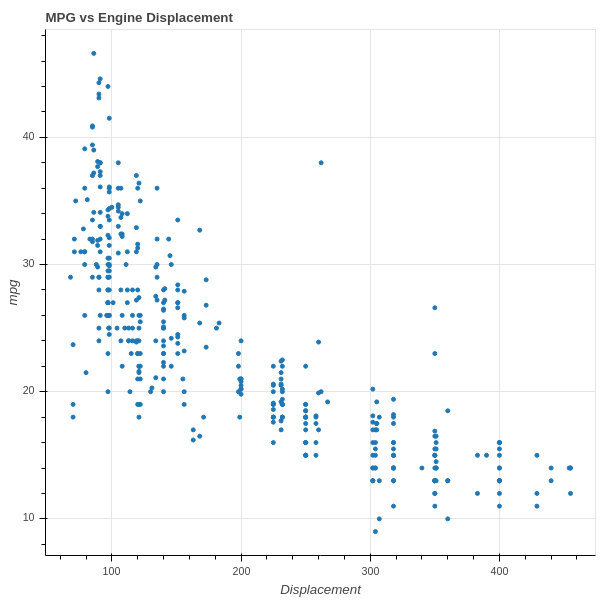
\includegraphics[width=3in,height=\textheight]{../img/mpg-vs-displacement.png}
\caption{Physics Experiment}\label{fig:dvt}
}
\end{figure}

On the other hand, we might look at a graph such as
\cref{fig:mpg-vs-displacement}, which plots the gas mileage of various
car models against their engine size (displacement), and observe a
general trend in which bigger engines get lower mileage. In this
situation we could ask for the best line of the form \(y=mx+b\) that
captures this relationship and use that to make general conclusions
without necessarily having an underlying theory.

\begin{figure}
\hypertarget{fig:mpg-vs-displacement}{%
\centering
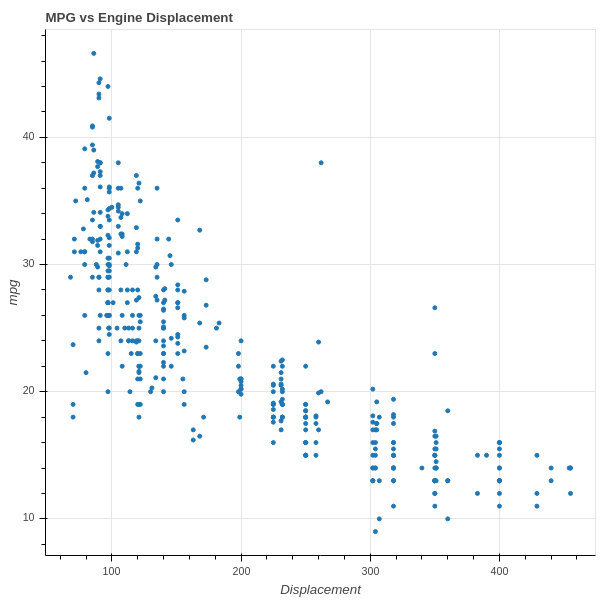
\includegraphics[width=3in,height=\textheight]{../img/mpg-vs-displacement.png}
\caption{MPG vs Displacement
({[}\protect\hyperlink{ref-irvine}{1}{]})}\label{fig:mpg-vs-displacement}
}
\end{figure}

\hypertarget{sec:Calculus}{%
\subsection{Least Squares (via Calculus)}\label{sec:Calculus}}

In either of the two cases above, the question we face is to determine
the line \(y=mx+b\) that ``best fits'' the data
\(\{(x_i,y_i)_{i=1}^{N}\}\). The classic approach is to determine the
equation of a line \(y=mx+b\) that minimizes the ``mean squared error'':

\[
MSE(m,b) = \frac{1}{N}\sum_{i=1}^{n} (y_i-mx_i-b)^2
\]

It's worth emphasizing that the \(MSE\) is a function of two variables
-- the slope \(m\) and the intercept \(b\) -- and that the data points
\(\{(x_i,y_i)\}\) are constants for these purposes. Furthermore, it's a
quadratic function in those two variables. Since our goal is to find
\(m\) and \(b\) that minimize the \(MSE\), we have a Calculus problem
that we can solve by taking partial derivatives and setting them to
zero.

To simplify the notation, let's abbreviate \(MSE\) by \(E\).

\[\begin{aligned}
\frac{\partial E}{\partial m} &= \frac{1}{N}\sum_{1}^{N}-2x_i(y_i-mx_i-b) \\
\frac{\partial E}{\partial b} &= \frac{1}{N}\sum_{1}^{N}-2(y_i-mx_i-b) \\
\end{aligned}
\]

We set these two partial derivatives to zero, so we can drop the \(-2\)
and regroup the sums to obtain two equations in two unknowns (we keep
the \(\frac{1}{N}\) because it is illuminating in the final result):

\begin{equation}
\begin{aligned}
\frac{1}{N}(\sum_{i=1}^{N} x_i^2)m &+& \frac{1}{N}(\sum_{i=1}^{N} x_i)b &=& \frac{1}{N}\sum_{i=1}^{N} x_i y_i \\
\frac{1}{N}(\sum_{i=1}^{N} x_i)m &+& b &=& \frac{1}{N}\sum_{i=1}^{N} y_{i} \\
\end{aligned}
\label{eq:LS}\end{equation}

In these equations, notice that \(\frac{1}{N}\sum_{i=1}^{N} x_i\) is the
average (or mean) value of the \(x_i\). Let's call this
\(\overline{x}\). Similarly, \(\frac{1}{N}\sum_{i=1}^{N} y_{i}\) is the
mean of the \(y_i\), and we'll call it \(\overline{y}\). If we further
simplify the notation and write \(S_{xx}\) for
\(\frac{1}{N}\sum_{i=1}^{N} x_i^2\) and \(S_{xy}\) for
\(\frac{1}{N}\sum_{i=1}^{N}x_iy_i\) then we can write down a solution to
this system using Cramer's rule:

\begin{equation}
\begin{aligned}
m &= \frac{S_{xy}-\overline{x}\overline{y}}{S_{xx}-\overline{x}^2} \\
b &= \frac{S_{xx}\overline{y}-S_{xy}\overline{x}}{S_{xx}-\overline{x}^2} \\
\end{aligned}
\label{eq:LSAnswer}\end{equation}

where we must have \(S_{xx}-\overline{x}^2\not=0\).

\hypertarget{sec:CalcExercises}{%
\subsubsection{Exercises}\label{sec:CalcExercises}}

\begin{enumerate}
\def\labelenumi{\arabic{enumi}.}
\item
  Verify that \cref{eq:LSAnswer} is in fact the solution to the system
  in \cref{eq:LS}.
\item
  Suppose that \(S_{xx}-\overline{x}^2=0\). What does that mean about
  the \(x_i\)? Does it make sense that the problem of finding the ``line
  of best fit'' fails in this case?
\end{enumerate}

\hypertarget{sec:LinAlg}{%
\subsection{Least Squares (via Geometry)}\label{sec:LinAlg}}

In our discussion above, we thought about our data as consisting of
\(N\) pairs \((x_i,y_i)\) corresponding to \(n\) points in the
\(xy\)-plane \(\mathbf{R}^2\). Now let's turn that picture ``on its
side'', and instead think of our data as consisting of \emph{two} points
in \(\mathbf{R}^{n}\):

\[
X=\left[\begin{matrix} x_1\cr x_2\cr \vdots\cr x_n\end{matrix}\right] \mathrm{\ and\ }
Y = \left[\begin{matrix} y_1\cr y_2\cr \vdots\cr y_n\end{matrix}\right]
\]

Let's also introduce one other vector

\[
E = \left[\begin{matrix} 1 \cr 1 \cr \vdots \cr 1\end{matrix}\right].
\]

First, let's assume that \(E\) and \(X\) are linearly independent. If
not, then \(X\) is a constant vector (why?) which we already know is a
problem from \cref{sec:Calculus}, Exercise 2. Therefore \(E\) and \(X\)
span a plane in \(\mathbf{R}^{n}\).

\begin{figure}
\hypertarget{fig:perp}{%
\centering
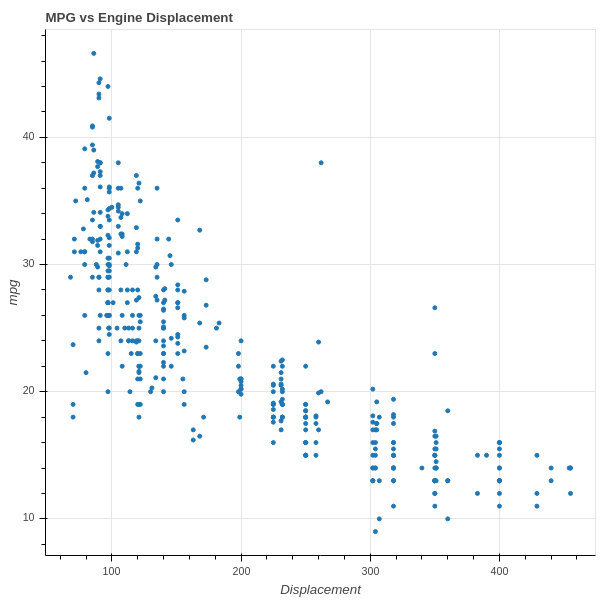
\includegraphics[width=3in,height=\textheight]{../img/mpg-vs-displacement.png}
\caption{Distance to A Plane}\label{fig:perp}
}
\end{figure}

Now if our data points \((x_i,y_i)\) all \emph{did} lie on a line
\(y=mx+b\), then the three vectors \(X\), \(Y\), and \(E\) would be
linearly dependent:

\[
Y = mX + bE.
\]

Since our data is only approximately linear, that's not the case. So
instead we look for an approximate solution. One way to phrase that is
to ask:

\emph{What is the point \(\hat{Y}\) in the plane \(H\) spanned by \(X\)
and \(E\) in \(\mathbf{R}^{n}\) which is closest to \(Y\)?}

If we knew this point \(\hat{Y}\), then since it lies in \(H\) we would
have \(\hat{Y}=mX+bE\) and the coefficients \(m\) and \(b\) would be a
candidate for defining a line of best fit \(y=mx+b\). Finding the point
in a plane closest to another point in \(\mathbf{R}^{n}\) is a geometry
problem that we can solve.

\textbf{Proposition:} The point \(\hat{Y}\) in the plane spanned by
\(X\) and \(E\) is the point such that the vector \(Y-\hat{Y}\) is
perpendicular to \(H\).

\textbf{Proof:} See \cref{fig:perp} for an illustration -- perhaps you
are already convinced by this, but let's be careful. \(\hat{Y}=mX+bE\)
such that \[
D = \|Y-\hat{Y}\|^2 = \|Y-mX-bE\|^2
\] is minimal. Using some vector calculus, we have \[
\frac{\partial D}{\partial m} = \frac{\partial}{\partial m} (Y-mX-bE)\cdot (Y-mX-bE) = -2(Y-mX-bE)\cdot X
\] and \[
\frac{\partial D}{\partial b} = \frac{\partial}{\partial b} (Y-mX-bE)\cdot (Y-mX-bE) = -2(Y-mX-bE)\cdot E.
\]

So both derivatives are zero exactly when \(\hat{Y}=(Y-mX-bE)\) is
orthogonal to both \(X\) and \(E\), and therefore every vector in \(H\).

We also obtain equations for \(m\) and \(b\) just as in our first look
at this problem.

\begin{equation}
\begin{aligned}
m(X\cdot E) &+ b(E\cdot E) &= (Y\cdot E) \cr
m(X\cdot X) &+ b(E\cdot X) &= (Y\cdot X) \cr
\end{aligned}
\label{eq:LSAnswer2}\end{equation}

We leave it is an exercise below to check that these are the same
equations that we obtained in \cref{eq:LSAnswer}.

\hypertarget{exercises}{%
\subsubsection{Exercises}\label{exercises}}

\begin{enumerate}
\def\labelenumi{\arabic{enumi}.}
\tightlist
\item
  Verify that \cref{eq:LSAnswer} and \cref{eq:LSAnswer2} are equivalent.
\end{enumerate}

\hypertarget{sec:Multivariate-calculus}{%
\subsection{The Multivariate Case
(Calculus)}\label{sec:Multivariate-calculus}}

Having worked through the problem of finding a ``line of best fit'' from
two points of view, let's look at a more general problem. We looked
above at a scatterplot showing the relationship between gas mileage and
engine size (displacement). There are other factors that might
contribute to gas mileage that we want to consider as well -- for
example: - a car that is heavy compared to its engine size may get worse
mileage - a sports car with a drive train that gives fast acceleration
as compared to a car with a transmission designed for long trips may
have different mileage for the same engine size.

Suppose we wish to use engine displacement, vehicle weight, and
acceleration all together to predict mileage. Instead of looking points
\((x_i,y_i)\) where \(x_i\) is the displacement of the \(i^{th}\) car
model and we try to predict a value \(y\) from a corresponding \(x\) as
\(y=mx+b\) -- let's look at a situation in which our measured value
\(y\) depends on multiple variables -- say displacement \(d\), weight
\(w\), and acceleration \(a\) with \(k=3\) -- and we are trying to find
the best linear equation

\begin{equation}
y=m_1 d + m_2 w + m_3 a +b
\label{eq:multivariate}\end{equation}

But to handle this situation more generally we need to adopt a
convention that will allow us to use indexed variables instead of \(d\),
\(w\), and \(a\). We will use the \emph{tidy} data convention.

\textbf{Tidy Data:} A dataset is tidy if it consists of values
\(x_{ij}\) for \(i=1,\ldots,N\) and \(j=1,\ldots, k\) so that:

\begin{itemize}
\tightlist
\item
  the row index corresponds to a \emph{sample} -- a set of measurements
  from a single event or item;
\item
  the column index corresponds to a \emph{feature} -- a particular
  property measured for all of the events or items.
\end{itemize}

In our case,

\begin{itemize}
\tightlist
\item
  the \emph{samples} are the different types of car models,
\item
  the \emph{features} are the properties of those car models.
\end{itemize}

For us, \(N\) is the number of different types of cars, and \(k\) is the
number of properties we are considering. Since we are looking at
displacement, weight, and acceleration, we have \(k=3\).

So the ``independent variables'' for a set of data that consists of
\(N\) samples, and \(k\) measurements for each sample, can be
represented by a \(N\times k\) matrix

\[
X = \left(\begin{matrix}
x_{11} & x_{12} & \cdots & x_{1k} \\
x_{21} & x_{22} & \cdots & x_{2k} \\
\vdots & \vdots & \ddots & \vdots \\
x_{N1} & x_{k2} & \cdots & x_{Nk} \\
\end{matrix}\right)
\]

and the measured dependent variables \(Y\) are a column vector \[
Y = \left[\begin{matrix} y_1 \\ y_2 \\ \vdots \\ y_N\end{matrix}\right].
\]

If \(m_1,\ldots, m_k\) are ``slopes'' associated with these properties
in \cref{eq:multivariate}, and \(b\) is the ``intercept'', then the
predicted value \(\hat{Y}\) is given by a matrix equation

\[
\hat{Y} = X\left[\begin{matrix} m_1 \\ m_2 \\ \cdots \\ m_k\end{matrix}\right]+\left[\begin{matrix} 1 \\ 1 \\ \cdots \\ 1\end{matrix}\right]b
\]

and our goal is to choose these parameters \(m_i\) and \(b\) to make the
mean squared error:

\[
MSE(m_1,\ldots, m_k,b) = \|Y-\hat{Y}\|^2 = \sum_{i=1}^{N} (y_i - \sum_{j=1}^{k}  x_{ij}m_j -b )^2.
\]

Here we are summing over the \(N\) different car models, and for each
model taking the squared difference between the true mileage \(y_i\) and
the ``predicted'' mileage \(\sum_{j=1}^{k} x_{ij}m_j +b\). We wish to
minimize this MSE.

Let's make one more simplification. The intercept variable \(b\) is
annoying because it requires separate treatment from the \(m_i\). But we
can use a trick to eliminate the need for special treatment. Let's add a
new feature to our data matrix (a new column) that has the constant
value \(1\).

\[
X = \left(\begin{matrix}
x_{11} & x_{12} & \cdots & x_{1k} & 1\\
x_{21} & x_{22} & \cdots & x_{2k} & 1\\
\vdots & \vdots & \ddots & \vdots & 1\\
x_{N1} & x_{k2} & \cdots & x_{Nk} & 1\\
\end{matrix}\right)
\]

Now our data matrix \(X\) is \(N\times(k+1)\) and we can put our
``intercept'' \(b=m_{k+1}\) into our vector of ``slopes''
\(m_1, \ldots, m_k,m_{k+1}\):

\[
\hat{Y} = X\left[\begin{matrix} m_1 \\ m_2 \\ \cdots \\ m_k \\ m_{k+1}\end{matrix}\right].
\]

and our MSE becomes

\[
MSE(M) = \|Y - XM\|^2
\]

where

\[
M=\left[\begin{matrix} m_1 \\ m_2 \\ \cdots \\ m_k \\ m_{k+1}\end{matrix}\right].
\]

The Calculus approach to minimizing the \(MSE\) is to take its partial
derivatives with respect to the \(m_{i}\) and set them to zero. Let's
first work out the derivatives in a nice form for later.

\textbf{Proposition:} The gradient of \(MSE(M)=E\) is given by

\begin{equation}
\nabla E = \left[\begin{matrix} \frac{\partial}{\partial m_1}E \\ \frac{\partial}{\partial m_2}E \\ \vdots \\ \frac{\partial}{\partial m_{k+1}}E\end{matrix}\right] =  -2 X^{\intercal}Y + 2 X^{\intercal}XM
\label{eq:gradient}\end{equation}

where \(X^{\intercal}\) is the transpose of \(X\).

\textbf{Proof:} First, remember that the \(ij\) entry of
\(X^{\intercal}\) is the \(ji\) entry of \(X\). Also, we will use the
notation \(X[j,:]\) to mean the \(j^{th}\) row of \(X\) and \(X[:,i]\)
to mean the \(i^{th}\) column of \(X\). (This is copied from the Python
programming language; the `:' means that index runs over all
possibilities).

Since \[
E = \sum_{j=1}^{N} (Y_j-\sum_{s=1}^{k+1} X_{js}M_{s})^2
\] we compute: \begin{equation}\begin{aligned}
\frac{\partial}{\partial m_t}E &= -2\sum_{j=1}^{N} X_{jt}(Y_{j}-\sum_{s=1}^{k+1} X_{js}M_{s}) \\
&= -2(\sum_{j=1}^{N} Y_{j}X_{jt} - \sum_{j=1}^{N}\sum_{s=1}^{k+1} X_{jt}X_{js}M_{s}) \\
&= -2(\sum_{j=1}^{N} X^{\intercal}_{tj}Y_{j} -\sum_{j=1}^{N}\sum_{s=1}^{k+1} X^{\intercal}_{tj}X_{js}M_{s}) \\
&= -2(X^{\intercal}[t,:]Y - \sum_{s=1}^{k+1}\sum_{j=1}^{N} X^{\intercal}_{tj}X_{js}M_{s}) \\
&= -2(X^{\intercal}[t,:]Y - \sum_{s=1}^{k+1} (X^{\intercal}X)_{ts}M_{s}) \\
&= -2(X^{\intercal}[t,:]Y - (X^{\intercal}X)[t,:]M)\\
\end{aligned}\label{eq:gradient}\end{equation}

Stacking up the different rows to make \(E\) yields the desired formula.

\textbf{Proposition:} Assume that \(D=X^{\intercal}X\) is invertible
(notice that it is a \((k+1)\times(k+1)\) square matrix so this makes
sense). The solution \(M\) to the multivariate least squares problem is
\[
M = D^{-1}X^{\intercal}Y
\] and the ``predicted value'' \(\hat{Y}\) for \(Y\) is \begin{equation}
\hat{Y} = XD^{-1}X^{\intercal}Y.
\label{eq:projection}\end{equation}

\hypertarget{the-multivariate-case-geometry}{%
\subsection{The Multivariate Case
(Geometry)}\label{the-multivariate-case-geometry}}

Let's look more closely at the equation obtained by setting the gradient
of the error, \cref{eq:gradient}, to zero. Remember that \(M\) is the
unknown vector in this equation, everything else is known:

\[
X^{\intercal}Y = X^{\intercal}XM
\]

Here is how to think about this:

\begin{enumerate}
\def\labelenumi{\arabic{enumi}.}
\item
  As \(M\) varies, the \(N\times 1\) matrix \(XM\) varies over the space
  spanned by the columns of the matrix \(X\). So as \(M\) varies \(XM\)
  is a general element of the subspace \(H\) of \(R^{N}\) spanned by the
  \(k+1\) columns of \(X\).
\item
  The product \(X^{\intercal}XM\) is a \((k+1)\times 1\) matrix. Each
  entry is the dot product of the general element of \(H\) with one of
  the \(k+1\) basis vectors of \(H\).
\item
  The product \(X^{\intercal}Y\) is a \((k+1)\times 1\) matrix whose
  entries are the dot product of the basis vectors of \(H\) with \(Y\).
\end{enumerate}

Therefore, this equation asks for us to find \(M\) so that the vector
\(XM\) in \(H\) has the same dot products with the basis vectors of
\(H\) as \(Y\) does. The condition

\[
X^{\intercal}\cdot (Y-XM)=0
\]

says that \(Y-XM\) is orthogonal to \(H\). This argument establishes the
following proposition.

\textbf{Proposition:} Just as in the simple one-dimensional case, the
predicted value \(\hat{Y}\) of the least squares problem is the point in
\(H\) closest to \(Y\) -- or in other words the point \(\hat{Y}\) in
\(H\) such that \(Y-\hat{Y}\) is perpendicular to \(H\).

\hypertarget{orthogonal-projection}{%
\subsubsection{Orthogonal Projection}\label{orthogonal-projection}}

Recall that we introduced the notation \(D=X^{\intercal}X\), and let's
assume, for now, that \(D\) is an invertible matrix. We have the formula
(see \cref{eq:projection}): \[
\hat{Y} = XD^{-1}X^{\intercal}Y.
\]

\textbf{Proposition:} The matrix \(P=XD^{-1}X^{\intercal}\) is an
\(N\times N\) matrix called the orthogonal projection operator onto the
subspace \(H\) spanned by the columns of \(X\). It has the following
properties:

\begin{itemize}
\tightlist
\item
  \(PY\) belongs to the subspace \(H\) for any \(Y\in\mathbf{R}^{N}\).
\item
  \((Y-PY)\) is orthogonal to \(H\).
\item
  \(P*P = P\).
\end{itemize}

\textbf{Proof:} First of all, \(PY=XD^{-1}X^{\intercal}Y\) so \(PY\) is
a linear combination of the columns of \(X\) and is therefore an element
of \(H\). Next, we can compute the dot product of \(PY\) against a basis
of \(H\) by computing

\[
X^{\intercal}PY = X^{\intercal}XD^{-1}X^{\intercal}Y = X^{\intercal}Y
\]

since \(X^{\intercal}X=D\). This equation means that
\(X^{\intercal}(Y-PY)=0\) which tells us that \(Y-PY\) has dot product
zero with a basis for \(H\). Finally,

\[
PP = XD^{-1}X^{\intercal}XD^{-1}X^{\intercal} = XD^{-1}X^{\intercal}=P.
\]

\hypertarget{exercises-1}{%
\subsubsection*{Exercises}\label{exercises-1}}
\addcontentsline{toc}{subsubsection}{Exercises}

\hypertarget{refs}{}
\leavevmode\hypertarget{ref-irvine}{}%
{[}1{]} \textsc{U.C. Irvine ML Repository}. Auto MPG Dataset.Available
at \url{http://https://archive.ics.uci.edu/ml/datasets/Auto+MPG}.

\end{document}
